\documentclass[12pt]{book}
                            % do not right justify
\usepackage[spanish]{babel}
\selectlanguage{spanish}
\usepackage[utf8]{inputenc}
\usepackage{geometry}
 \geometry{
 a4paper,
 total={170mm,257mm},
 left=20mm,
 top=20mm,
 }
% \bibliography{biblio}

\title{Navindoor: Software para la simulación, desarrollo y validación de sistemas de localización}    % Supply information
\author{Deyviss Jesús Oroya Villalta}              %   for the title page.
\date{\today}                           %   Use current date. 

% Note that book class by default is formatted to be printed back-to-back.
\begin{document}                        % End of preamble, start of text.
\frontmatter                            % only in book class (roman page #s)
\maketitle                              % Print title page.
\tableofcontents                        % Print table of contents
\mainmatter                              % only in book class (arabic page #s)
% \chapter*{Introducción}
\addcontentsline{toc}{chapter}{Introducción}

% Introdución a posicionamiento 
% Descripcion de la diversidad de tecnologias 

% Introducion al problema
    % - Modelos dependientes del entorno
    % - Dificil Comparación entre métodos 
    % - 

% Simulacion como solucion al problema 


% S

% \chapter{Sistemas de posicionamiento en interiores}

% -
\section{Clasificación de IPS}


\subsection{Triangulación mediante RSS y ToF}

% Yang, Jie; Chen, Yingying (2009-11-01). Indoor Localization Using Improved RSS-Based Lateration Methods. IEEE Global Telecommunications Conference, 2009. GLOBECOM 2009. pp. 1–6. CiteSeerX 10.1.1.386.4258. doi:10.1109/GLOCOM.2009.5425237. ISBN 978-1-4244-4148-8.

% Kotaru, Manikanta; Joshi, Kiran; Bharadia, Dinesh; Katti, Sachin (2015-01-01). SpotFi: Decimeter Level Localization Using WiFi. Proceedings of the 2015 ACM Conference on Special Interest Group on Data Communication. SIGCOMM '15. New York, NY, USA: ACM. pp. 269–282. 
\subsection{Trilateración mediante AoA}

\subsection{Fingerprinting}

% [1] P. Bahl and V. N. Padmanabhan, “RADAR: an in-building RF-based user location and tracking system,” in Proceedings of 19th Annual Joint Conference of the IEEE Computer and Communications Societies (INFOCOM ’00), vol. 2, pp. 775–784, Tel Aviv.Israel, March 2000.

% [3] Youssef, M. A.; Agrawala, A.; Shankar, A. Udaya (2003-03-01). WLAN location determination via clustering and probability distributions. Proceedings of the First IEEE International Conference on Pervasive Computing and Communications, 2003. (PerCom 2003). pp. 143–150. CiteSeerX 10.1.1.13.4478. doi:10.1109/PERCOM.2003.1192736. ISBN 978-0-7695-1893-0.

La toma de huellas dactilares tradicional también se basa en RSSI, pero simplemente se basa en el registro de la intensidad de la señal desde varios puntos de acceso en el rango y el almacenamiento de esta información en una base de datos junto con las coordenadas conocidas del dispositivo cliente en una fase fuera de línea. Esta información puede ser determinista [1] o probabilística. [3] Durante la fase de seguimiento en línea, el vector RSSI actual en una ubicación desconocida se compara con los almacenados en la huella dactilar y la coincidencia más cercana se devuelve como la ubicación estimada del usuario. Estos sistemas pueden proporcionar una precisión media de 0,6 my una precisión de la cola de 1,3 m. [8] [10]

Su principal desventaja es que cualquier cambio en el entorno, como agregar o quitar muebles o edificios, puede cambiar la "huella digital" que corresponde a cada ubicación, lo que requiere una actualización de la base de datos de huellas digitales. Sin embargo, la integración con otros sensores, como la cámara, se puede utilizar para hacer frente a los cambios en el entorno.

Campo magnético, Barómetro, 
\subsection{Sistemas Inerciales}
% \chapter{Descripción de la plataforma Navindoor}\label{S3}

\section{Estado del arte}\label{S2}
Los simuladores son una gran herramienta para mejorar el diseño, prueba y validación de sistemas de localización. Es por ello que podemos encontrar distintos intentos en la comunidad científica. A continuación se resumirán algunos trabajos existentes en el ámbito, además de describir sus principales características.

% ----------------------------------------------------
SMILe   es una herramienta de simulación de código abierto, para desarrollar y evaluar métodos de localización en interiores basados en el tiempo de propagación como métricas de localización, tales como el Tiempo de Vuelo (ToF) o la Diferencia de Tiempo de Llegada (TDoA). Esta herramienta está basada en el simulador OMNET+++ y un paquete de funcionalidades escritas en Python para el análisis y el procesamiento de datos. SMILe permite al usuario configurar un espacio, donde se pueden cambiar varios factores que afectan significativamente el rendimiento de la localización. Estos factores incluyen el despliegue de diferentes nodos, capacidades de radio y la inexactitud de relojes.
% Comparación Navindoor  

Tanto en Navindoor como en SMILe existen herramientas necesarias para el diseño, prueba y evaluación de algoritmos de localización a partir de ToF. Sin embargo, mientras que en SMILe señales de otra índole todavía no están contempladas, en Navindoor se abarca más diversidad de tecnologías. Aun así, el modelo de simulación de señales de ToF de SMILe es más complejo que el modelo de simulación de Navindoor. 
% ----------------------------------------------------

PyLayers es un simulador de radio frecuencia de código abierto. Se ha diseñado para evaluar el rendimiento de algoritmos de localización. El canal de radio se sintetiza mediante el uso de un  método de trazado de rayos basado en gráficos. El movimiento de personas se modela con un enfoque de fuerzas virtuales. Los datos simulados se pueden procesar directamente con uno de los algoritmos de localización incorporados o se pueden exportar a varias extensiones para el procesamiento externo. 
% Comparación Navindoor   

Al igual que en el caso anterior, PyLayers contiene un simulador complejo para una tecnología concreta. Aunque ofrece la posibilidad de procesar las señales dentro del propio simulador, hace énfasis en la exportación de sus resultados para el procesamiento externo. En Navindoor, se opta por ofrecer un interfaz para la incorporación de nuevos modelos de simulación, manteniendo todo el proceso en un mismo entorno de desarrollo.
% ----------------------------------------------------

% pro
\emph{Sensor Fusion and Tracking Toolbox}  es una biblioteca desarrollada por Mathworks que incluye algoritmos y herramientas para diseñar, simular y analizar sistemas que fusionan datos de varios sensores con el objetivo de hacer seguimiento de la posición y orientación de objetos.
Esta biblioteca incluye funcionalidades para la generación de trayectorias y escenarios, simular mediciones de sensores inerciales (acelerómetro, giroscopio, magnetómetro), receptores de GPS, radar, sonar e infrarrojo, diferentes algoritmos de fusión y estimación (filtros de Kalman y filtros de partículas), y herramientas para visualizar, analizar y comparar el rendimiento de los diferentes algoritmos.

% Comparación Navindoor  
En esta biblioteca, al igual que en Navindoor, se provee de herramientas en todo el proceso de diseño de sistemas de localización. Sin embargo, en \emph{Sensor Fusion and Tracking Toolbox} por ahora solo se ha desarrollado una  CLI, careciendo de GUI. Por otra parte, los modelos de simulación en la generación de trayectorias son generales, no simulan un activo en concreto. En Navindoor los modelos de simulación están enfocados al movimiento de personas.

\section{Navindoor}
% - Características generales
Navindoor ha sido desarrollado bajo el paradigma de la programación orientada a objetos. Se han definido clases para representar elementos en el diseño de sistemas de localización. La planimetría, las trayectorias o las señales son clases que contiene métodos asociados para su visualización, la extracción de datos e interacción entre ellos. Por otro lado, tenemos los algoritmos de localización y las métricas para comparar algoritmos. Estas están representadas por funciones que actúan sobre las clases antes mencionadas.
% - Funcionales
%     - Proceso de experimentación en sistemas de localización -> arquitectura modular
%     - Incluye modelos y algoritmos por defecto pero preparado para incluir nuevos
%     - Guardar/Cargar datos

Estas clases y funciones se han desarrollado en cinco módulos que siguen el proceso de experimentación en el diseño de sistemas de localización. Para tener una visión global de ello, se describirá brevemente este proceso y el módulo propuesto en cada punto:

\begin{enumerate}
    \item \textbf{Obtención de la planimetría.} El primer paso en la experimentación es la elección del escenario y la obtención de la planimetría de este. En Navindoor, se ha creado el módulo de planimetría con la clases necesarias para construir una planimetría de varios niveles. 
    %
    \item \textbf{Generación de trayectorias.} En la experimentación, se toman puntos de referencia para poder construir trayectorias a través de ellas. Esto limita la variedad de las trayectorias, sin embargo es necesario para obtener medidas precisas de la posición en cada instante. 
    %
    En Navindoor se ha creado el módulo de generación de trayectorias, dedicado a la simulación de trayectorias. Debido a que estamos en un entorno de simulación tenemos información exacta sobre la trayectoria real, generada a partir de una sucesión de puntos proporcionada por el usuario.
    %
    %
    \item \textbf{Toma de medidas de señales.} En la experimentación, una vez generada la trayectoria, se debe enriquecer esta con señales. El tercer módulo, llamado modulo de generación de señales, ésta dedicado a la simulación de señales sintéticas. Gracias a la simulación, podemos crear las señales después de haber sido generada la trayectoria. 
    %
    %
    \item \textbf{Procesamiento de señales.} Tras la toma de medidas, los algoritmos de localización se encargan de procesar las señales. El cuarto módulo de Navindoor, llamado módulo de procesamiento de medidas, provee algoritmos capaces de crear estimaciones de la trayectoria real a partir de las señales simuladas. Además de ofrecer un esquema donde nuevos algoritmos puedan ser desarrollados.
    %
    %
    \item \textbf{Comparación de Algoritmos.} Por último, para poder validar los algoritmos desarrollados es necesario la comparación con otros algoritmos ya consolidados. El quinto módulo de Navindoor es el módulo de validación de algoritmos, que nos provee de métodos de comparación de algoritmos proporcionados por el usuario o entre algoritmos por defecto.
\end{enumerate}
% - Técnicas
%     - Framework/API y GUI
%     - Requisitos: Matlab R2017b?
% - URL donde está disponible Navindoor
Dentro de estos módulos se encuentran repartidas las clases y funciones definidas en Navindoor. Cabe mencionar que tanto el CLI, como el GUI son compatibles en versiones de MATLAB superiores a MATLAB R2017b y se encuentran disponibles en .

A continuación se expondrán los detalles de cada uno de los módulos.


\subsection{Módulo de planimetría}

% A- Módulo de planimetría
% - Objetivo del módulo	
El objetivo de este módulo es caracterizar el escenario donde transcurre el experimento. Actualmente las trayectorias en Navindoor se centran en el desplazamiento en interiores, por lo que se ofrecen las herramientas básicas para caracterizar un edificio de varias plantas. Esta caracterización nos proveerá información sobre las restricciones de movimiento, posición de puntos de acceso, altura entre plantas, etc. Esta información puede ser usada por los modelos generación de trayectorias y señales, además de los algoritmos de localización.
% - Modelización 
%     - Diagrama de clases
%     - nodos, paredes, puertas, ascensores, escaleras, APs, plantas

Se ha diseñado una jerarquía de clases presentada en la figura \ref{fig:esquemabuilding}, que representan los objetos necesarios para la caracterización de un edificio. Se ha creado la clase \emph{node}, para representar un punto en el espacio tridimensional. A partir de este objeto se construyen las demás clases dentro del módulo de planimetría. Los objetos \emph{walls}, que representa  las paredes del edificio, se construyen a partir de dos objetos \emph{node}. Por otra parte, también existen  elementos puntuales, por lo que se han creado clases que heredan las propiedades de \emph{node}. Estos son los objetos \emph{stairs}, \emph{elevators}, \emph{doors} y \emph{beacons}. Los objetos \emph{stairs} y \emph{elevators} indican los puntos de salida de una planta. Los objetos \emph{doors}, se definen dentro de los objetos \emph{wall}s, y permiten el paso en su entorno. Por último, los objetos \emph{beacons} representan puntos de acceso generadores de señales de radio frecuencia. Los objetos antes mencionados se almacenan en una clase llamada \emph{level} en forma de atributos. Por último se ha creado la clase \emph{building} que en sus atributos contiene una lista de objetos \emph{level}. 
\begin{figure}[!ht]
    \centering
    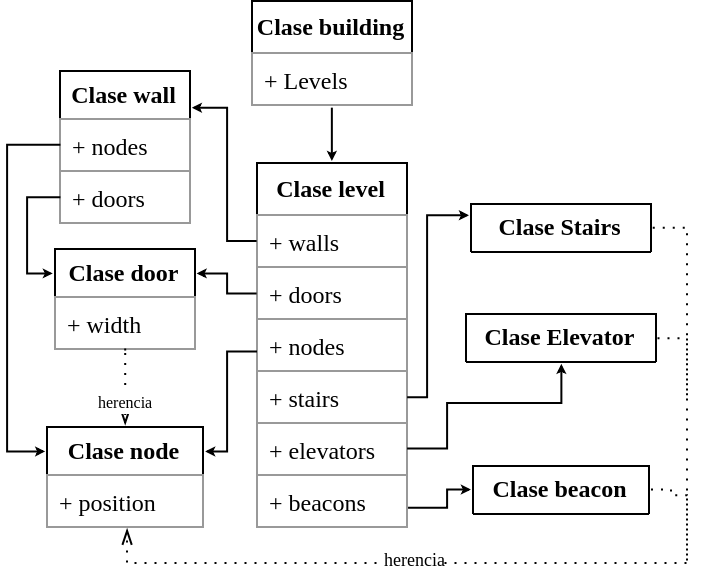
\includegraphics[width=0.5     \columnwidth]{img/Design/planimetria.png} 
    \caption[]{Esquema de la clases.}
    \small
    Las flechas salientes indican de qué clase es el objeto. Mientras que el listado dentro de cada caja representa las propiedades que contiene una clase. 
    \label{fig:esquemabuilding}
\end{figure}   


% - Explicación básica del proceso de generación de planimetría:  
%     - Clicks con el ratón 
%     - mapa real como plantilla
%     - Visualización 3D
Para la creación de cada uno de estos objetos existe un constructor siguiendo las bases de la programación orientada a objetos, sin embargo la caracterización de la planimetría de esta forma puede ser muy tediosa. Es por ello que se ha optado en el desarrollo de una GUI (figura \ref{fig:interfaz1}), que nos ayude en este trabajo. De esta forma se puede definir objetos \emph{nodes} con simples \emph{clicks}, y paredes uniendo objetos \emph{nodes}. Además la GUI permite cargar imágenes, en formato PNG, de la planimetría de interés dentro del espacio de trabajo. Esto se puede realizar para cada una de las plantas de manera que podamos crear una fiel reproducción de la planimetría utilizando los planos reales como plantillas. Un vez construido la planimetría podemos ver el objeto \emph{building} en 3D, gracias a las opciones de la GUI.


\begin{figure}
    \centering
    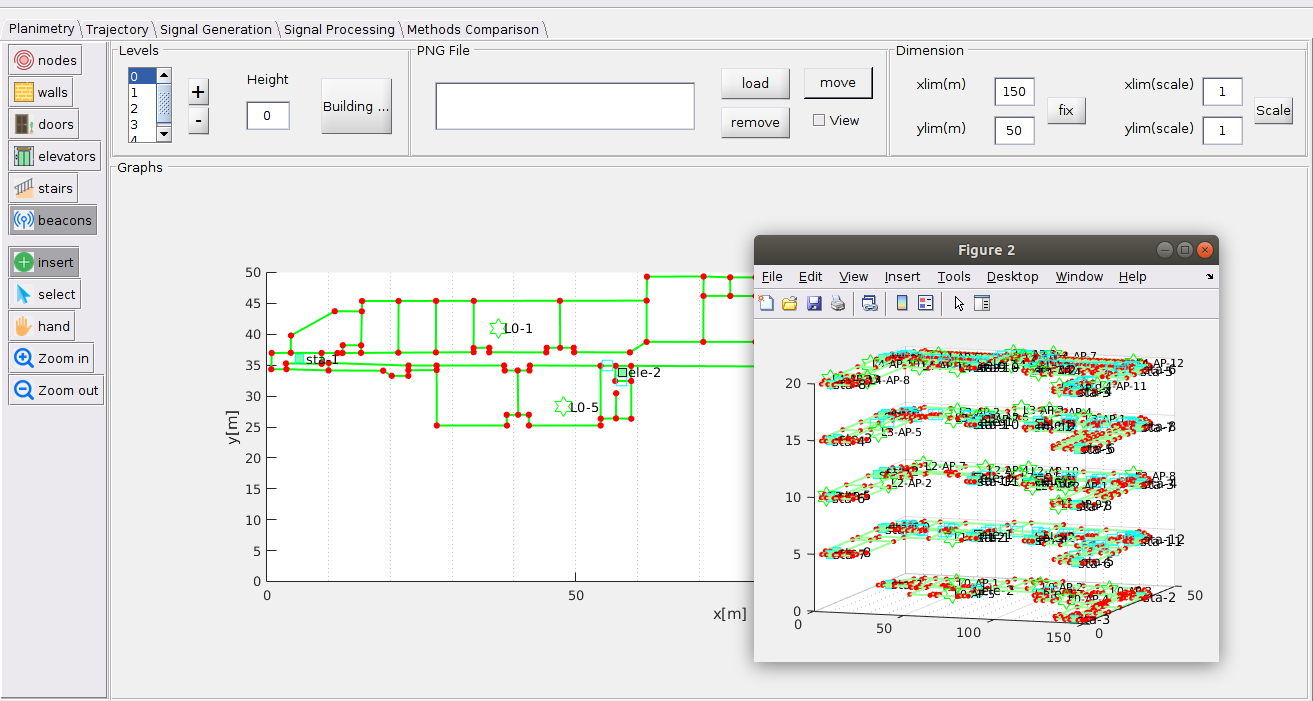
\includegraphics[width=1.00\columnwidth]{img/Design/1.PNG}
    \caption{Interfaz gráfica para el diseño de la planimetría \emph{building}.}
    \small
    En la imagen se muestra la interfaz con un edificio de cinco plantas. La figura externa es una representación tridimensional del edificio.
    \label{fig:interfaz1}
\end{figure}

% ----------------------------------------------------------------------


\subsection{Módulo de generación de trayectorias}

% B- Módulo de generación de trayectorias
% - Objetivo del módulo	
El objetivo de este módulo es generar trayectorias dentro de la planimetría creada. La modelización de las trayectorias permite conseguir una vista preliminar del comportamiento de los algoritmos. Los modelos de movimiento toman importancia en este módulo, ya que de ello dependerá la similitud de los resultados obtenidos con la realidad.
% - Modelización
%       - trayectoria

En Navindoor, las trayectorias están modeladas como una sucesión de puntos dentro de la planimetría. Estos puntos definen los tramos por donde se moverá el activo. Estos se pueden definir con la ayuda de GUI, simplemente haciendo \emph{click} dentro de la planimetría, incluyendo los cambios de planta.

Un vez definidos los puntos por donde pasará el activo, con ayuda de modelos de simulación se genera una sucesión de puntos más fina. Esta contiene  coordenadas de los puntos, además del instante de tiempo correspondiente. De esta forma, las velocidades y aceleraciones se pueden obtener mediante diferenciación. Los modelos de generación de la trayectorias en nuestro caso están centrados en la simulación del pie de una persona, por lo que se simulan medidas de los sistemas inerciales \emph{foot-mounted}. En concreto se utiliza el modelo propuesto en . Además en los casos de cambios de planta se agrega un modelo de velocidad constante.

A partir de la  trayectoria del pie de la persona, se genera la trayectoria del centro de masas. Esta se usará en los casos en el que el sensor esté sobre el tronco de la persona. En la figura se muestra el proceso para la generación de un objeto trayectoria. 

Es importante notar que tanto los modelos de simulación de la trayectoria del pie, como el modelo de generación de la trayectoria del centro de masas, son parámetros opcionales. Es decir, los modelos de simulación son independientes de Navindoor, por lo que nuevos modelos pueden ser implementados creando funciones con la misma interfaz de entrada/salida que las funciones ofrecidas por defecto.

Por último, en la GUI tenemos herramientas para la generación de la trayectoria, desde la opción para crear una sucesión de puntos con \emph{clicks}, pasando por la creación de nuevos modelos, hasta la visualización de la trayectoria generada (figura \ref{fig:animation}).

\begin{figure}[ht!]
    \centering
    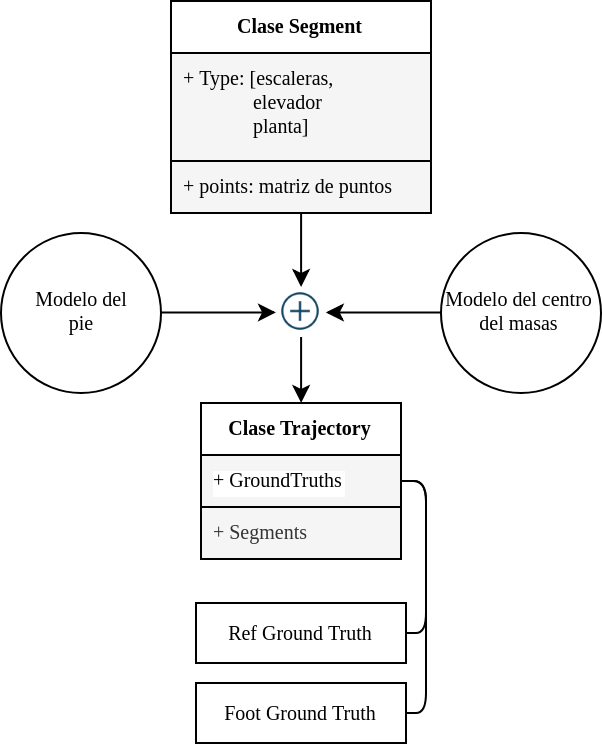
\includegraphics[width=0.75\columnwidth]{img/Design/trajectory.png}
    \caption{Proceso de construcción de una trayectoria.}
    \label{TrajectorySch}
    \small
    En este esquema se puede ver cómo el constructor de la trayectoria, genera dos objetos \emph{GroundTruths} a partir de segmentos que contienen información extraída de la planimetría. Además, es necesario un modelo que construya la trayectoria del pie de una persona a través de los segmentos y un modelo que sea capaz de crear la trayectoria del centro de masas a partir de la trayectoria del pie. El objeto \emph{Ref GroundTruth} representa la trayectoria del centro de masas, mientras que \emph{Foot GroundTruth} representa la trayectoria del pie de la persona.
\end{figure}



%       - Explicación básica del proceso de generación de trayectorias: 
%       - Selección planta
%       - Clicks con el ratón
%       - Comprobación paredes
%       - Paso a otras plantas
%   - Animación 3D

\begin{figure}
    \centering
    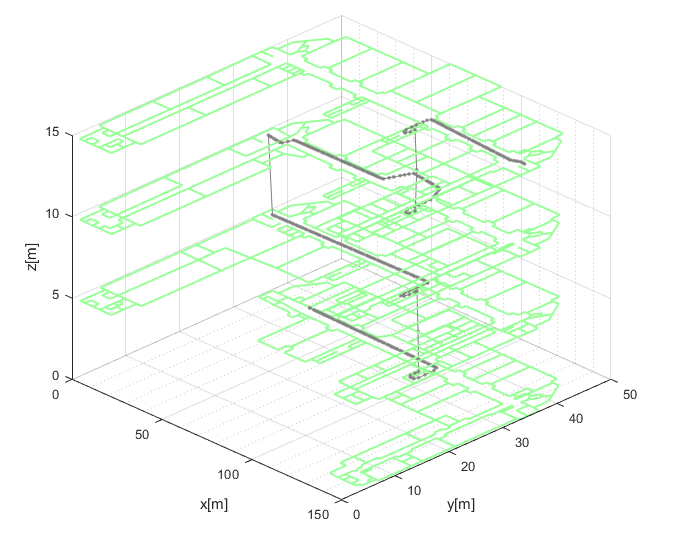
\includegraphics[width=0.8\columnwidth]{img/Design/untitled.png}
    \caption[]{Captura de una animación de una trayectoria}
    \label{fig:animation}
    \small
    Esta tiene su inicio en la planta cinco y baja usando distintas escaleras y ascensores hasta la primera planta.
\end{figure}


% ----------------------------------------------------------------------
\subsection{Módulo de generación de señales}

% C- Módulo de generación de medidas asociadas a una trayectoria
% - Objetivo del módulo		
En este módulo se podrán simular distintos tipos de señales a partir de la trayectoria generada. El objetivo es generar datos que los algoritmos de localización procesarán. Al igual que en el módulo anterior, los modelos de simulación son cruciales para que el comportamiento del simulador sea fiel a la realidad. 

% - Modelización	
%     - Tipos de señales y métricas			
En Navindoor se ha creado la clase abstracta \emph{Signal} con propiedades que contiene la información de las medidas a lo largo de un periodo de tiempo. Además, se han creado dos clases que heredan los métodos y propiedades de la clase \emph{Signal}. Estas son:
\begin{itemize}
    \item La clase \emph{BeaconBased}: Representando señales que necesitan  puntos de acceso para poder ser simuladas. 
    \item La clase \emph{BeaconFree}: Representando señales que pueden ser simuladas sin la necesidad de los puntos de acceso.
   \end{itemize}

Dentro del entorno de simulación, las diferencias entre estas clases se ven en la forma de construirlas. Mientras que la clase \emph{BeaconFree}, solo necesita la información de la trayectoria para ser definida, la clase \emph{BeaconBased} necesita los objetos \emph{beacons} definidos en el módulo de la planimetría (figura \ref{schemaBB}). 

La clase \emph{BeaconBased} puede representar señales de atenuación de nivel de potencia (RSS), ángulo de llegada (AoA) y tiempo de vuelo (ToF), mientras que la clase \emph{BeaconFree} puede representar señales inerciales (aceleraciones lineales y velocidades angulares), intensidades de campo magnético y presión atmosférica. Los modelos de simulación de señales utilizados por defecto son básicos con una componente de ruido gaussiano.

% \begin{table}[ht]
%     \centering
%     \begin{tabular}{|c|c|}
%         \hline
%         {\textbf{BeaconBased}} & {\textbf{BeaconFree}}          \\ \hline
%         {Atenuación de nivel de potencia (RSS)}    & Barómetro        \\ \hline
%         {Tiempo de vuelo (ToF)}              & Acelerómetro               \\ \hline
%         {Angulo de llegada (AoA)}            & Magnetómetro             \\ \hline
%                                             & giroscopio             \\ \hline

%     \end{tabular}
%     \caption{Tipo de modelos de simulación de señales}
%     \label{tiposenales}
% \end{table}


En Navindoor se trata a los modelos como parámetros de entrada, por lo que es posible cambiarlos por modelos más complejos simplemente creando funciones con una interfaz de entrada/salida específica. En el caso de las clases \emph{BeaconBased}, los parámetros de entrada deberán ser un punto de la trayectoria y un objeto \emph{beacon}; y dar como parámetro de salida el valor de la señal. Mientras que en el caso de la clase \emph{BeaconFree}, solo se usa un punto de la trayectoria como parámetro de entrada y el valor de la señal como parámetro de salida.

%     - Diagrama de clases
\begin{figure}[ht!]
    \centering
        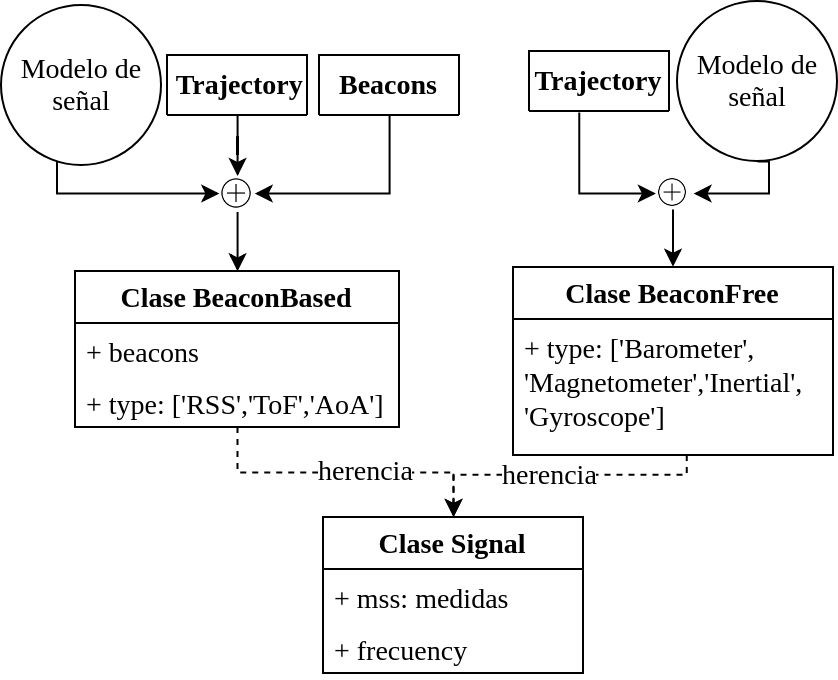
\includegraphics[width=0.85\columnwidth]{img/Design/signaldiagram.png}
        \caption{Representación de la generación de las señales.}
        \small
        Se muestra un esquema de la generación de las señales \emph{BeaconFree} y \emph{BeaconBased}. Además, también se muestra la clase \emph{Signal} de la cual heredan las propiedades donde estarán las medidas.
        \label{schemaBB}
    \end{figure} 

 

% - Explicación básica del proceso de generación de medidas asociada a una trayectoria: 
%     - Modelos de ruido: parámetros, crear modelos nuevos
%     - Visualizar señal generada
Por la parte de la GUI, en Navindoor se ha implementado un apartado para la generación de señales. En esta se muestra un listado de trayectorias previamente generadas. También se muestra un selector donde poder elegir el tipo de señal que queramos generar. Para cada uno de estos tipos nos enseña un listado de los modelos existentes. Además nos permite crear nuevos modelos a partir de una plantilla para cada tipo de señal. De esta manera dentro de la GUI podemos crear varias señales rápidamente, además de visualizar el resultado obtenido. 

% \begin{figure}[ht!]
%     \centering
%         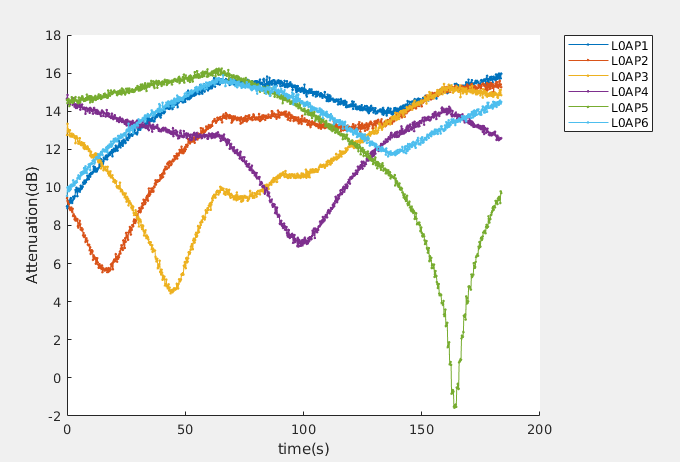
\includegraphics[width=1.0\columnwidth]{img/Design/GUIsignal.png}
%         \caption{Visualización de una señal generada en navindoor}
%         \small
%         \label{graphsBB}
%     \end{figure}


\subsection{Módulo de procesamiento de medidas}
% ----------------------------------------------------------------------
% D- Módulo de estimación de la trayectoria
% - Objetivo del módulo	
El objetivo de este módulo es proveer al usuario algoritmos básicos para la localización a partir de las señales generadas. Estos algoritmos se utilizarán como punto de partida para el diseño de nuevos. 

% - Interfaz de los algoritmos de localización
En Navindoor se encuentra implementados  el filtro de Kalman extendido (EKF)y el Filtro de Kalman \emph{Unscented} (UKF) . Para implementar nuevos algoritmos es necesario que estos tengan una interfaz de entrada/salida específica. Los algoritmos deberán tener tres parámetros de entrada: El objeto \emph{building}, una lista de las señales generadas en todos los instantes de tiempo y una estructura con toda la información a \emph{priori} de la trayectoria. Además deberán tener como parámetro de salida una matriz de cuatro columnas. Las tres primeras columnas indicando el espacio y la última columna el tiempo (figura \ref{format}). Navindoor se encarga de procesar esta información para crear un objeto trayectoria. De esta manera la estimación contará con las propiedades y métodos de la trayectoria real.  
\begin{figure}[ht!]
    \centering
        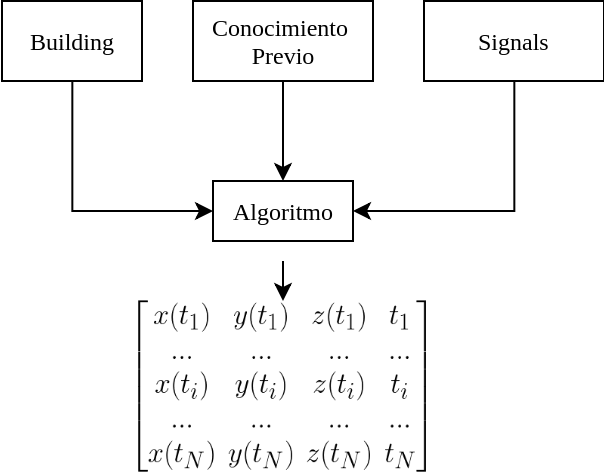
\includegraphics[width=0.725\columnwidth]{img/Design/InterfazAlgo.png}
        \caption{Interfaz de entrada/salida para los algoritmos de localización}
        \small
        Como entrada tiene tres variables, la primera representando la planimetría, la segunda representado todo el conocimiento previo sobre la trayectoria y el tercero un listado de las señales. El algoritmo devuelve una matriz $4 \times N$, siendo N el número de medidas
        \label{format}
    \end{figure}

% - Explicación básica del procesado de medidas y estimación de la trayectoria
Con respecto a la GUI, Navindoor muestra un listado de las trayectorias que han sido generadas. Para cada una de estas trayectorias podemos ver las señales disponibles. De esta manera podemos seleccionar la trayectoria y las señales que queramos procesar. Dado que los algoritmos tienen el interfaz entrada/salida antes presentado, es posible ejecutarlos con un solo \emph{click}. Navindoor, luego de ejecutar el algoritmo muestra la trayectoria real y la trayectoria estimada dentro de la planimetría cargada. Además gracias a que la estimación es un objeto trayectoria, podemos utilizar la animación utilizada en el módulo de generación de trayectorias, dando una visión a tiempo real del comportamiento de la trayectoria real frente a la trayectoria estimada.



\subsection{Módulo de evaluación de algoritmos}

% E- Módulo de evaluación
% - Objetivo del módulo			
El objetivo de este último módulo es comparar distintas estimaciones de la trayectoria. La diferencia de las ejecuciones puede estar en el algoritmo utilizado para estimar, sin embargo también puede estar en los modelos de simulación de la trayectoria, en los modelos simulación de señales, o simplemente en la frecuencia de muestreo de alguna señal. Deberemos notar que las estimaciones en Navindoor son objetos trayectorias por lo que desde el punto de vista del código, no existe diferencia estructural entre la trayectoria real y la estimación. Esto hace que la comparación entre ellas sea más fácil.
% - Explicación básica de la evaluación y comparación de rendimiento de los algoritmos

En la GUI, Navindoor nos muestra una lista de las trayectorias generadas, pudiendo seleccionar una de ellas. Para cada una de estas trayectorias se muestran las estimaciones disponibles. Podemos seleccionar las estimaciones que queramos para compararlas en un mismo gráfico representando la función de distribución acumulada empírica (eCDF), tomando como referencia la trayectoria real. De esta forma tenemos una visión del comportamiento de las dos estimaciones en un mismo gráfico.

\chapter{Implementación de modelos de simulación y algoritmos de localización}


\section{Filtros de Kalman}
\subsection{Modelo Dinámico de un peatón}

El movimento de un peatón puede modelizarse como un movimento rectilineo a velocidad constante en variaciones de tiempos muy pequeños. 

\begin{gather}\label{MRU}
    \frac{d}{dt}
    \begin{pmatrix}
        x \\ y \\ z \\
        u \\ v \\ w 
    \end{pmatrix} = 
    \begin{pmatrix}
        u \\ v \\ w \\
        0 \\ 0 \\ 0       
    \end{pmatrix}
\end{gather}

Podemos discretizar la ecuación (\ref{MRU}) mediante el método de euler. Dado que resolveremos la ecuación en intervalos temporales muy pequeños con respecto a la variación de la velocidad de un peatón no necesitamos más precisión. 

\begin{gather} 
    \begin{pmatrix} \label{MRUDis}
        x \\ y \\ z \\
        u \\ v \\ w 
    \end{pmatrix}_{k+1} =
    \begin{pmatrix}
        1 & 0 & 0 & dt & 0  & 0 \\
        0 & 1 & 0 & 0  & dt & 0 \\
        0 & 0 & 1 & 0  & 0  & dt \\
        0 & 0 & 0 & 1  & 0  & 0 \\
        0 & 0 & 0 & 0  & 1  & 0 \\
        0 & 0 & 0 & 0  & 0  & 1 \\
    \end{pmatrix}
    \begin{pmatrix}
        x \\ y \\ z \\
        u \\ v \\ w     
    \end{pmatrix}_k
\end{gather}

El paso temporal, $dt$ debido a la discretización será igual que la latencia del algoritmo de predicción.




\subsection{Modelo de medidas de balizas} 

Supongamos que tenemos $n$ balizas. Además las posiciones de estas balizas estan contenidas en una  matriz $M_b \in \mathcal{M}_{3 \times n}(\mathbb{R})$. Podemos definir una función, $h(M_b)$ dada la matriz, $M_b$. Sea una función $h(M_b): \R^3 \rightarrow    \R^{n \times m}$ tal que recibe un punto del espacio, $r \in \R^3$ y devuelve un vector de medidas, $z \in \R^{n \times m}$.

\begin{gather}
    \begin{array}{llll}
        h(M_b):  & r     & \rightarrow & M_m \\
            & \R^3  & \rightarrow & \mathcal{M}_{n \times m}(\R)    
    \end{array}
\end{gather}









\section{Fusión de señales para la estimación de la trayectoria mediante filtros de Kalman}


%\chapter{Conclusiones}




% \addcontentsline{toc}{chapter}{\textbf{Biblografía}}
% \printbibliography
\end{document}                          % The required last line 